	
	% XeLaTeX can use any Mac OS X font. See the setromanfont command below.
	% Input to XeLaTeX is full Unicode, so Unicode characters can be typed directly into the source.

	% The next lines tell TeXShop to typeset with xelatex, and to open and save the source with Unicode encoding.

	%!TEX TS-program = xelatex
	%!TEX encoding = UTF-8 Unicode

	\documentclass[12pt,a4paper]{article}
	\usepackage{geometry}                % See geometry.pdf to learn the layout options. There are lots.
	\geometry{letterpaper}                   % ... or a4paper or a5paper or ... 
	%\geometry{landscape}                % Activate for for rotated page geometry
	%\usepackage[parfill]{parskip}    % Activate to begin paragraphs with an empty line rather than an indent
	\usepackage{graphicx}
	\usepackage{amssymb}
	\usepackage{url}
	\usepackage{listings}
	\lstset{
	language=Perl, 
	basicstyle=\footnotesize,       % the size of the fonts that are used for the code
	numbers=left,                   % where to put the line-numbers
	numberstyle=\footnotesize,      % the size of the fonts that are used for the line-numbers
	stepnumber=1,                   % the step between two line-numbers. If it's 1 each line will be numbered
	numbersep=5pt,                  % how far the line-numbers are from the code
	backgroundcolor=\color{white},  % choose the background color. You must add \usepackage{color}
	showspaces=false,               % show spaces adding particular underscores
	showstringspaces=false,         % underline spaces within strings
	showtabs=false,                 % show tabs within strings adding particular underscores
	frame=single,	                % adds a frame around the code
	tabsize=2,	                % sets default tabsize to 2 spaces
	captionpos=b,                   % sets the caption-position to bottom
	breaklines=true                % sets automatic line breaking
	}



	\usepackage[usenames,dvipsnames]{color}
	% Will Robertson's fontspec.sty can be used to simplify font choices.
	% To experiment, open /Applications/Font Book to examine the fonts provided on Mac OS X,
	% and change "Hoefler Text" to any of these choices.

	\usepackage{fontspec,xltxtra,xunicode}
	\defaultfontfeatures{Mapping=tex-text}
	%\setromanfont[Mapping=tex-text]{Helvetica Neue}
	%\setsansfont[Scale=MatchLowercase,Mapping=tex-text]{Gill Sans}
	%\setmonofont[Scale=MatchLowercase]{Andale Mono}
        \setmainfont{Liberation Sans}
        % \setmonofont{Liberation Mono}

	\title{\textbf{Cataloguing genomic polymorphisms \\ using NGS} }
	\author{TSL training course \\\\ Christian Schudoma\\\texttt{christian.schudoma@tsl.ac.uk}}
	\date{}                                           % Activate to display a given date or no date

	\begin{document}
	\maketitle
	\begin{center}
	%\includegraphics[width=90mm]{NEED A COVER PICTURE }
	\end{center}
	\pagebreak
	\tableofcontents
	\pagebreak
	


\section{Cataloguing polymorphisms in genomes with next-generation sequencing}

We will go through the individual steps of using Illumina sequences
from two bulk accessions of \emph{Solanum}, one susceptible to a
pathogen (BS) and the other resistant (BR). We will create a sequence
alignment against a small \emph{Solanum} reference sequence, analyse
the data for indels and SNPs, and view them in Galaxy's Trackster
Genome Browser

\subsection{Why look for SNPs?}

\textbf{S}ingle-\textbf{N}ucleotide \textbf{P}olymorphisms (SNPs) are
variations in a DNA sequence that occur when a single nucleotide in a
genome is changed. A SNP may lead to a change in function or
expression of a gene. SNPs may form premature stop codons, form a
different fold in a given protein, or alter gene expression. SNPs can
also be used as genetic markers, linking a gene to a given trait and
can be used to study the response of a host to a pathogen.

\subsection{Getting started with Galaxy}

Go to \texttt{http://galaxy.tsl.ac.uk/}.\\

Login using your username and password. If you are using a training
account (e.g. \texttt{b26stu10@nbi.ac.uk}), start off by making sure
that all the histories (possibly left over from previous training
courses) are deleted. At the top right hand corner of the page at the
top of the history panel click on the options wheel and click on Saved
Histories. A list of currently active histories should be displayed in
the central console. There should only be one history - called
'Unnamed History'. If there is more than one, check all the boxes next
to the histories and then click on 'Delete' at the bottom of the page.

\subsection{Getting the data}

We will begin by accessing the data to use in the tutorial.
\begin{enumerate}
	\item First, create a new named history. If your current
          history is called 'Unnamed History' click on the name and
          type in a history name that makes sense, e.g. 'SNP training
          course'. Hit return to save the new name.
	\item From the Galaxy homepage, you will see 6 menus across
          the top of the page, the third of which should read 'Shared
          Data'. Click on this menu item and a drop down list of
          options should appear, the first of which should read 'Data
          Libraries'. Click on 'Data Libraries'.
	\item In the list of Data Libraries you will see one called
          'tsl training'. Click on this and you will see a couple of
          subfolders. Next to the folder 'SNP detection' click on the
          blue arrow-head and check the boxes next to
          '\emph{Solanum}\_reference.fasta', 'BR\_left.fastqsanger',
          'BR\_right.fastqsanger', 'BS\_left.fastqsanger' and\\
          'BS\_right.fastqsanger'. Make sure 'Import to current
          history' is selected in the box below and click on
          'Go'. Click on 'Analyze Data' in the menu to return to the
          main interface.
	\item You will be taken back to your homepage where you should
          see the four fastq files and one fasta file in your history.
\end{enumerate}

\subsection{Quality Control}

Illumina sequencing is not 100\% accurate. Errors are introduced
during sequencing and base-calling have a degree of uncertainty, which
is encoded in the fastq quality scores.  \\

Quality controlling (QC) reads involves a number of steps: joining
paired-end sequences together, removing sequences with N's, removing
sequences that are not exactly twice the length of a single-end read,
examining the per-base quality of the reads and trimming or removing
reads that have low quality scores. Time spent making sure you have
good quality data at the start of your experiments will be time saved
at the end, filtering out spurious results that are caused by
low-quality reads.  \\ 

There are a number of ready-made workflows for quality controlling in
Galaxy. If you would like to use them, just contact me and I will put
you on the right track.\\ 

The data we are using today has already been quality controlled so
there is no need to carry out these steps.

\section{Mapping with BWA}

We will now map our Illumina reads to the \emph{Solanum} reference
sequence using the BWA next-generation sequence aligner.

\subsection{BWA}

BWA is a next-generation sequence aligner used to map relatively short
sequences to a reference genome. It uses the Burrows-Wheeler Transform
(BWT, \\
see also \texttt{http://en.wikipedia.org/wiki/Burrows–Wheeler\_transform}) to
reduce the amount of memory needed to align reads by creating a
compressed index of the reference sequence. It is designed for short
queries up to \textasciitilde200bp with low error rate ($<$3\%) and is
very fast.

\begin{enumerate}
	\item Click on 'NGS: Mapping' in the toolbox and from the
          expanded list select 'Map with BWA for Illumina'.  \\

          There are lots of options to be aware of in BWA. We will
          start at the top of the page and work down. First of all, we
          need to select the reference sequence to map our reads
          to. As we have loaded our reference from the data library
          and it is not a pre-loaded build, make sure the first drop
          down box reads 'Use one from the history' and that the
          reference genome is 'Solanum\_reference.fasta'. Then
          we need to tell Galaxy what type of reads we have. Selecting
          'Paired-end' from the next drop down list will refresh the
          page and drop-down lists for the forward and reverse files
          will appear. We have two sets of reads (BS and BR) and each
          set of reads has a left-reads and a right-reads file. We
          want to map each set separately in order to compare them
          later so we'll start by mapping the BS reads first. For the
          'Forward FASTQ file:' select your left-hand reads file
          (BS\_left.fastqsanger in this case) and then the right-hand
          reads (BS\_right.fastqsanger) for the 'Reverse FASTQ file:'.

	\item Next we will look at the BWA advanced settings. Click on
          the 'BWA settings to use' list and change it from 'Commonly
          Used' to 'Full Parameter List'.

	\item We will see a long list of parameters appear below -
          here is what some of them mean. The 'Maximum edit distance'
          is the maximum number of nucleotides in a read that can
          mis-match with the reference and the read still be
          aligned. This number can be given as a fraction in the next
          field instead. The 'Maximum number of gap opens' field
          refers to the amount of insertions that can occur across a
          read. 'Disallow insertion/deletion within [value] bp towards
          the end' refers to the fact that sequence quality
          deteriorates towards the end of a sequence and the user
          might not want to trust indels in the last few bases of a
          read. One parameter we might want to change is the
          second-to-last one - 'Maximum insert size for a read pair to
          be considered as being mapped properly:'. The insert size of
          reads is the distance between the outer ends of the two
          paired-end reads. This is part of the initial experimental
          design and refers to the size of the fragment cut out of the
          gel for sequencing. The insert size for our reads is 400
          nucleotides, so we would expect that the distribution of
          insert-sizes should not exceed 500nt. Make sure the value is
          500 and hit 'Execute'.
	\item Now, repeat steps 1-3 above using the bulk-resistant
          (BR) reads instead of the BS reads.
	\item When finished mapping both sets of data, rename the
          output files to 'BS.sam' and 'BR.sam' by clicking on the
          pencil icon next to the name of the history item.
\end{enumerate}

\section{Finding SNPs}

\subsection{SAM format}

We now have our reads mapped to the \emph{Solanum} reference. The
output format from BWA is SAM (Sequence Alignment/Map) format. The SAM
format describes the alignment of sequenced reads to a reference
sequence. It stores all the alignment information generated by BWA in
a simple and compact format. It provides information about the
position of the read in relation to the reference genome, the number
and position of nucleotides that match to the genome and the position
of indels. We can use the SAM file to take a closer look at our
alignment.\\

Click on the output 'Map with BWA for Illumina...' file and view the
SAM format output file. The first few lines start with '@SQ SN'
followed by the name of the sequences in the reference file
(chromosome names in this case) and the length of the sequence. Then
there will be a line beginning with '@PG'. Because the SAM format is
generic, it is used by a number of different next-gen sequence
aligners. The @PG line gives us information about the program name
(PN) used to produce the alignment and what version (VN) was used.\\ 

Every line after that corresponds to each read that BWA
handled. Each line starts with the name of the read and has a number
of columns of data after it. In the 3rd column we can see which
chromosome our read has been mapped to and the position of the first
mapped base in column 4. An unmapped read will have a * in column 3
and zero in column 4. The 5th column is the mapping quality, a score
quantifying the probability that a read is misplaced. The next column
is the CIGAR string and consists of numbers followed by an upper-case
letter (the operator). Many of the CIGAR strings will read '76M'. This
means that in the current alignment of the read against the reference,
all 76 nucleotides of the read match (M) the reference. Some other
operators we might find in the CIGAR string are 'I' meaning an
insertion to the reference, 'D' meaning a deletion from the reference
and 'S' meaning soft-clipping, where part of the read, usually at the
start or end of the alignment, does not match the reference. \\

As an example, a CIGAR string of 36M3D40M means 36 matching
nucleotides, followed by 3 deletions and ending in 40 matches.  \\

Take a look at the CIGAR strings in the SAM file. What combinations
of CIGAR string can you find? Compare the mapping quality values of
reads that have a CIGAR string of 76M to those that have a different
combination - what do you notice about the mapping qualities?  \\

More information on the SAM format can be found via the following
link: \\

\texttt{http://samtools.sourceforge.net/}

\subsection{SAM to BAM}

A BAM file is a highly compressed, indexed binary version of SAM and
through a library of different tools, allows fast, random access to
the alignment.
\begin{enumerate}
	\item The next step in the analysis requires us to change our
          SAM file into a binary BAM file. This is a simple
          step. Click on 'NGS: SAM Tools' and then click
          'SAM-to-BAM'. We will need to tell the program that we are
          using a reference in the history, so select 'History' from
          'Choose the source for the reference list:' and then make
          sure our \emph{Solanum}\_reference is selected in the 'Using
          reference file:'. In the 'Convert SAM file' select the SAM
          file which you want to convert (as earlier, we will handle
          the BS file first and then BR later). Hit 'Execute'.
	\item The output of this step will be a BAM file. You will
          not be able to view this file in Galaxy as it is a
          compressed binary file.
	\item Again, rename your history items, this time to 'BS.bam'
          and 'BR.bam'.
\end{enumerate}

\subsection{Creating an MPileup}

\subsubsection{MPileup format}

The MPileup format is a per-line base-by-base representation of the
alignment. It provides a much more coherent way of viewing the
alignment. The first three columns represent the reference name,
position on the reference and the reference base. After that there are
another three columns for each alignment in the pileup - read depth,
bases, and base qualities.  \\
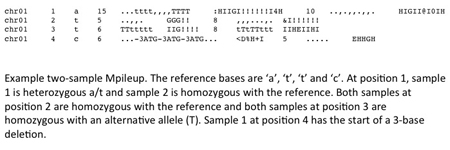
\includegraphics{images/mpileup.jpg}
\begin{enumerate}
	\item Now that we have our BAM files we can create an
          MPileup. In the toolbox, click on 'NGS: SAM Tools' and then
          'MPileup'.
	\item As with many other tools, there are a number of options
          we need to consider when using this tools. Firstly though,
          we need to tell MPileup what data we want to use. Select
          'History' in the 'Choose the source for the reference list:'
          and select the \emph{Solanum} reference sequence. This is
          the point in our experiment that we combine our alignments,
          so want to use both of our BAM files.  \\Select our BS.bam
          file in the first 'BAM files' field and then click on 'Add
          new BAM file' and select the BR.bam file in the BAM file 2
          field.
	\item Under 'Set advanced options:' select 'Advanced' and
          notice the extra parameters appear. Now we have a range of
          options to look at. Firstly, above the 'Advanced' field
          there is the 'Genotype Likelihood Computation:' field. We
          will leave that set to 'Do not perform genotype likelihood
          computation'. Changing it to perform genotype likelihood
          computation is used to directly perform snp and indel
          calling and it provides a very different output (compressed
          BCF format) to what we require. Read down the list of
          parameters. Some of them are straight-forward, some are
          not. 'Coefficient for downgrading mapping quality for reads
          containing excessive mismatches' assigns a read a lower
          mapping quality if it contains excessive mismatches to the
          reference sequence. A zero value disables this
          functionality; if enabled, the recommended value for BWA is
          50. 'Max reads per BAM' is the number of reads examined
          before the consensus base is called.  A couple of parameters
          refer to 'BAQ' - per-Base Alignment Quality, which
          accurately measures the probability of a read base being
          wrongly aligned. Using BAQ greatly reduces false SNP calls
          caused by misalignment around insertions and deletions
          (indels) by downgrading quality scores if a misalignment is
          likely. 'Extended BAQ computation' helps sensitivity
          especially for multiple nucleotide polymorphisms (MNPs), but
          may hurt specificity a little bit. There are two parameters
          that refer to minimum mapping quality and minimum base
          quality. 'Base quality' refers to the fact that each base call
          is an estimate of the true nucleotide. It is a random
          variable and can be wrong. Base qualities are encoded in the
          Phred-scale and originate in the fastq sequence. They are
          generally in the range between 1 (very bad) and 40 (very
          good). 'Mapping quality' refers to the probability that a read
          alignment can be wrong. It takes into account the repeat
          structure of the reference (reads falling in repetitive
          regions usually get very low mapping quality), the base
          quality of the read (low quality means the observed read
          sequence is possibly wrong, and wrong sequence may lead to a
          wrong alignment), the sensitivity of the alignment algorithm
          (the true hit is more likely to be missed by an algorithm
          with low sensitivity, which also causes mapping errors) and
          whether the read is paired end or not (reads mapped in pairs
          are more likely to be correct). Once you're satisfied that
          you have the correct parameters set (just use the default
          parameters here), hit 'Execute'.
	\item Once the history item has turned green, click on the eye
          symbol to display the first few hundred lines of the
          Mpileup. We can see 9 columns. The first 3 columns represent
          information about the \emph{Solanum} reference sequence that
          we have mapped to - reference name, position and reference
          base. After that there are 3 columns for each of the two
          samples - coverage, read bases over the current position and
          base qualities for each base. At the read base column, a dot
          stands for a match to the reference base on the forward
          strand, a comma for a match on the reverse strand,
          \texttt{'ACGTN'} for a mismatch on the forward strand and
          \texttt{'acgtn'} for a mismatch on the reverse strand. A
          pattern \texttt{'+[0-9]+[ACGTNacgtn]+'} indicates there is
          an insertion between this reference position and the next
          reference position. Also at the read base column, a symbol
          \texttt{'\textasciicircum'} marks the start of a read
          segment. The ASCII-code of the character following
          \texttt{'\textasciicircum'} minus 33 gives the mapping
          quality. A symbol \texttt{'\$'} marks the end of a read
          segment.
\end{enumerate}

\section{Finding SNPS}

\subsection{VarScan}

Today we are going to use the VarScan tool to look for SNPs (and
later, indels). VarScan takes as input an MPileup file and examines
one base at a time, computing the number of bases supporting each
observed allele. Only bases meeting certain criteria (discussed below)
are considered.
\begin{enumerate}
	\item In the Galaxy Tool Panel go to VarScan > VarScan -
          mpileup2snp. The aim of mpileup2snp is to use a combination
          of heuristics and statistics to filter positions in the
          Mpileup file that look like variants. We will be quite
          conservative with the parameters so that we can identify as
          many variants as possible and then use a custom filter in a
          further step to extract the types of variants we are
          interested in.
	\item In the 'MPileup File' dropdown list, select your MPileup
          file from the previous step (make sure to select the MPileup
          file and not the log-file).
	\item We can now set a number of parameters to say how
          stringent we want to be when calling variants. Two of the
          parameters - 'Minimum coverage' and 'Minimum variant allele'
          can be filtered further in the next step, so we can leave
          those as they are. A 'Minimum variant allele' value of 0.01
          means that a variant will be called if 1\% of the read bases
          differ from the reference base. Similarly, the 'Minimum
          frequency to call homozygote' value of 0.75 means that 75\%
          of the bases must be identical to the reference base (or the
          alternate allele base) in order to be called homozygous. The
          'P-value threshold for calling variants' is calculated using
          Fisher's Exact Test on the read counts supporting reference
          and variant alleles. Using the 'Strand filter' tells VarScan
          to ignore variant calls where 90\% of the variant bases are
          on one strand. VarScan can output 2 types of format: basic
          tab-delimited results, or VCF format. We want our output in
          VCF format, so make sure 'Output VCF format' is checked and
          hit 'Execute'.
\end{enumerate}

\subsection{VCF format}

The output of VarScan is in Variant Call Format (VCF). Click on the
eye symbol of the output file to view it. \\ Although the VCF format
looks quite confusing, it is actually quite straightforward. \\

The lines starting with '\#\#' are the meta-data lines. They contain
key-value pairs separated by an '=' sign (e.g. number=1, Type=Integer,
Description="Some description"). To best describe the format, let us
start a bit further down the file at the only line to start with a
single '\#'. After the single \# you will see some uppercase column
headers called CHROM, POS, ID, REF, ALT and QUAL.  CHROM and POS refer
to the reference name and position of the SNP. REF is the reference
base and ALT refers to the variant base(s) at that position. The next
field we come across is 'FILTER'. FILTER is defined in our meta-data,
so take a look at the \#\#FILTER lines and this describes the meaning
of any entry which does not contain 'PASS' (PASS refers to the fact
that it has passed any filtering). We can see that there are two
possible alternatives to PASS: 'str10 and 'indelError'. The meaning of
'str10' is given in the Description 'Less than 10\% or more than 90\%
of variant supporting reads on one strand'. This means that if we did
not check the strand-filter during VarScan, then any positions that
had less than 10\% or more than 90\% of variant supporting reads on
one strand, would have been included but annotated by 'str10' in the
FILTER field.  \\ 

The next two fields are INFO and FORMAT and this is where the VCF
format really makes use of its meta-data. The information in the INFO
column will be a combination of key=value pairs, separated by
semi-colons. An entry will read something like
'ADP=27;WT=0;HET=2;HOM=0;NC=0'. Each key (e.g. ADP) will have its
meaning explained in the metadata \#\#INFO fields. If we look for
'ADP' in the metadata \#\#INFO fields we can see that there should
only be a single value (Number=1), it should be an integer
(Type=Integer), and that the value refers to "Average per-sample depth
of bases with Phred score >= 15". Note: the required Phred score in
this case is 15 as this was the value that we had in the VarScan
Minimum Quality field. If we'd change the Minimum Quality field to
'20', then the Description of the ADP field would read "Average
per-sample depth of bases with Phred score >= 20". Take a look at the
WT, HET, HOM and NC fields and understand their meaning.

Next is the FORMAT field. This reads slightly different from the INFO
field. All the keys of the key-value pairs are bunched together,
separated by colons,
e.g. 'GT:GQ:SDP:DP:RD:AD:FREQ:PVAL:RBQ:ABQ:RDF:RDR:ADF:ADR'. \\Again,
the meaning of these keys can be found in the meta-data in the
\#\#FORMAT lines. Each of these keys provides information about the
samples (i.e. BS (Sample1) and BR (Sample2)), and for each sample we
find the values of the preceeding keys. Take a look at the first
FORMAT key - 'GT'. We can see from the meta-data that GT stands for
genotype and if we look at the values of GT under the samples we can
see that there are three possible values: 0/0, 1/1 and 0/1. VarScan
estimates the genotype for each sample at each variant position. The
three values have the following meanings: 
\\* 0/0 - Homozygous to the reference (REF) 
\\* 1/1 - Homozygous to the alternate non-reference allele (ALT) 
\\* 0/1 - Heterozygous (0/2 represents a heterozygote with two
alternate alleles)

Take a look at the other key-value pairs and try to learn their
meaning from the meta-data.

The full specifications of VCF can be found here:   

\texttt{http://www.1000genomes.org/wiki/Analysis/Variant\%20Call\%20Format/\\vcf-variant-call-format-version-41}

\subsection{Filtering the VCF data}

Now that we understand what the data in our VCF file means, we can try
and filter it to get at what we're really interested in. In todays
experiment we're going to say that our BS sample should be homozygous
to the reference (so have a genotype of 0/0) and BR should be
heterozygous (0/1). As that information is in the VCF file, we'll use
a custom filter to extract the positions that match the required
genotypes.
\begin{enumerate}
	\item From the tool panel select VCF Tools > Filter VCF
          Genotypes.
	\item Under VCF file: select your VarScan mpileup2snp file   
	\item We can now apply a few parameters to be more stringent
          as to what we want to call a SNP. Firstly, we will increase
          the 'Minimum coverage' parameter. Earlier in VarScan we used
          a minimum coverage of 8, but now we are going to be a bit
          more stringent about what we want to filter out.  For our
          experiment today, as we are using a condensed training
          dataset, we will use a cut-off of 50. Normally, we would
          probably use something much higher than this. This parameter
          depends on various factors, one of which would be the
          sequencing . Next, we will set our minimum alternative
          allele frequency ('Alt allele frequency') frequency to
          0.2. The alternative allele frequency is calculated as the
          fraction of the alternative bases over all bases:
          $f_{alt} = \frac{alt}{alt+reference}$. \\
        \item Uncheck 'Strand filter' if it is checked. We already
          accounted for avoiding strand bias when using VarScan.
	\item Now we need to choose the combination of genotypes we
          are looking for. In this case we are looking for positions
          that are homozygous to the reference for BS and heterozygous
          for BR. It is probably not necessary to change the first
          'Genotypes to filter' field. The given sample name in the
          VCF file output by VarScan should be 'Sample1' and this
          should be our BS sample. However, we can (and should) use
          the 'New Sample Name' field to label our data with a more
          informative title. Instead of having 'Sample1' in the output
          we will have 'BS'. Make sure 'Genotype' is set to
          'homozygous with ref'.
	\item Click on 'Add new Genotypes to filter' to get another
          genotype filter. This time we want to handle the BR data,
          called 'Sample2' in the VCF file, so change the Sample Name
          to 'Sample2' and insert 'BR' in 'New Sample Name'. This time
          we want to look for heterozygous genotypes, so select the
          correct Genotype. Hit 'Execute'.
\end{enumerate}

The tool takes the VCF file output from VarScan, looks for positions
where the Sample1 (BS) is homozygous to the reference and Sample2 (BR)
is heterozygous. When it finds such a position, it checks that the
coverage is equal to or greater than 50 and whether the alt allele (if
searching for a heterozygote) is present at a frequency greater than
0.2. A position that meets all these criteria is added to the output
files.

This tool outputs two files - the first called 'Filter VCF Genotypes
on data x' and the other called 'Filter VCF Genotypes SNPs on data
x.bed'. View the first file. This is a list of our SNPs. Each SNP
position has one line per sample. As we have two samples, we have two
lines per SNP. It starts with the position of the SNP, the types of
the ref and alt bases, provides the genotype for the current sample
and then goes on to give further information about the sample such as
read depth, read quality, base counts, alt allele frequency and the
FET p-value. The second file is a BED file, a condensed annotation
file that we will use later to visualise our SNPs.

\subsection{SNP Confirmation}

The next step after filtering a list of SNPs might be to design
primers and use Sanger sequencing to confirm the presence of the
predicted SNPs in your accession of \emph{Solanum}.

\section{Finding Indels}

\subsection{Indels}

When comparing reads to a reference sequence, an insertion is one or
more 'extra' nucleotides inserted into the read and a deletion is one
or more nucleotides deleted from the read. Insertions and deletions
are called \emph{indels} and can occur anywhere in the genome. Unless
the length of the indel is a multiple of 3 (the length of a codon), it
can produce a frameshift mutation. We will use our alignment to look
for indels to identify where these potential frameshits occur.

When we mapped our reads with BWA, we allowed insertions and deletions
(indels) to be introduced into the alignments. The occurrences of
indels can be found in the SAM CIGAR string, indicated by the 'I' and
'D' operators. These indels were also kept in the MPileup file.  For
example a 2-nucleotide insertion of 'AG' is represented by '+2AG' in
the read base column and a 4-base deletion of CACC is represented by
'-4CACC'. Again, we can use VarScan to extract the indels from our
data.

\begin{enumerate}
	\item Select the VarScan > VarScan mpileup2indel tool.   
	\item Rather like what we did with the mpileup2snp tool, we
          will select our mpileup file and set the parameters that we
          wish to provide to the program, but this time we will be
          quite stringent from the start as there is no second-phase
          of filtering afterwards. We will start with the 'Minimum
          Coverage' field. We will use a coverage cut-off of 50 and
          set the 'Minimum Supporting Reads' parameter to 10. We will
          then change the 'Minimum variant allele' (indel) to 0.2. Leave
          the remaining values as they are and hit 'Execute'.
	\item As with the VarScan mpileup2snp tool the output of this
          tool should be in VCF format. Take a look at the output and
          you will see the indels in the ALT column.
	\item Finally, use the tool VarScan > vcf2bed. This tool turns
          a VCF file into a BED file (like the second output file of
          the Filter Genotypes tool), which is used for annotation.
\end{enumerate}

\section{SNP and indel visualisation}

\subsection{Trackster}

Not only is Galaxy a great analysis tool, it is also very good for
visualisation. It has an inbuilt visualisation tool called
Trackster. We will use Trackster to visualise the SNPs and indels that
we found during our experiment.

\subsection{Creating a new build}
\begin{enumerate}
	\item Using the top menu in Galaxy, click on Visualization >
          New Track Browser
	\item You will be presented with the New Visualisation box. We
          need to create what we call in Galaxy a 'build'. A build is
          a reference genome that is built into Galaxy. Sometimes
          builds are already available, but if they are not we have to
          build our own.
	\item Near the bottom of the box you will see 'Is the build
          not listed here? Add a Custom Build'. Click on 'Add a Custom
          Build'.
	\item You will be presented with the Add Custom Build
          page. Under 'New Build' use 'Solanum' in the 'Name' field
          and 'Solanum v1' in the 'Key' field. Make sure your
          \emph{Solanum} fasta reference sequence is selected under
          'Definition' and and hit Submit (see below).
	\item Your build should appear in the 'Current Custom Builds'
          at the top of the page.  \\
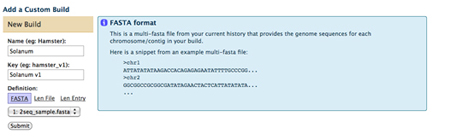
\includegraphics{images/custombuild.jpg}
\end{enumerate}

\subsection{Creating a new visualisation}
\begin{enumerate}
        \item Go back to the Galaxy home page and have a look at your
          history. We want to visualise our read alignments (the two
          BAM files, we created earlier) to the reference, as well as
          our annotated SNPs and indels (the two bed files).  For that
          we need to associate the respective files with the reference
          sequence. In the history, you will see the attribute
          'database: ?' for each file, click the '?' and choose your
          newly created custom build from the 'Database/Build' list.
	\item Now click on Visualization > New Track Browser again.
	\item Give your visualisation browser a name, e.g. 'Solanum
          browser' and select your new build from the 'Reference
          genome build (dbkey):' drop-down list.
	\item You should now be presented with a blank browser. At the
          top of the browser, click on the 'Add Datasets to
          Visualisation' button.
	\item The 'Select datasets for new tracks' page will
          appear. The data we want to look at is in our history, so
          click on the grey 'Histories' tab and then click on the name
          of your current history. You will see all the data in the
          current history that can be viewed in Trackster. %We want to
          %look at our sequence alignments, our snp annotations and our
          %indel annotations. To load the sequence alignments, check
          %the boxes next to the two BAM files that we created
          %earlier. The snp annotation file is the .bed file that we
          %created with the Genotype filter tool and the indel
          %annotation file is the bed file we created with the VarScan
          %vcf2bed tool. Check these two files and then click on 'Add'.
          Check all items and then click on 'Add'. 
	\item The genome browser will reappear. At the top of the page
          there is a drop-down list called 'Select
          chrom/contig'. Click on this and you should see the names of
          the two chromosomes in the reference sequence - 'chr01' and
          'chr02'. Click on 'chr01'.
	\item You will see the alignments appear on the page along
          with the annotation showing you where the snps and indels
          are. You can zoom into locations with the magnifying glass
          at the top of the page, or you can edit the co-ordinates by
          clicking on the current range (next to the drop-down list of
          references) and typing in your own coordinates. Coordinates
          use the following synax: chr:start-end. Note the colon
          between the chromosome/contig name and the hyphen between
          the start and end location, e.g. chr01:1000-1999. You can
          also zoom into an area by dragging across the region at the
          top of the page, where the coordinates are shown in larger
          intervals.
\end{enumerate}


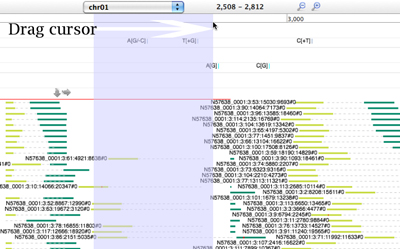
\includegraphics{images/DragZoom.jpg}

\subsection{Navigating the browser}
\begin{enumerate}
	\item Next to each dataset there are some settings that you
          can change. Hover your mouse over the name of one of the BAM
          files and the settings will appear. Try clicking on some of
          them and playing around with the settings (but don't click
          on the right-hand most 'x' - this removes the dataset).
	\item Zoom into a region which is annotated with a SNP. Scroll
          down through the aligned reads. Can you see the
          polymorphisms in the reads? Sometimes if there is a lot of
          coverage over that position, only the first few reads will
          be shown. If a yellow '!' triangle appears when you hover
          over the dataset name, you can click on the triangle to
          reveal more reads.
	\item Do the same for an indel. Insertions are annoted by a
          number in the reads, corresponding to the amount of inserted
          bases. The BED annotation file should show what these bases
          are. Deletions are annotated by a red line in the middle of
          the read.
	\item Finally, you can bookmark any interesting SNPs or
          indels. At the bottom right-hand corner of the page you will
          see a '$<$' symbol. Click on this and a new panel will open
          up on the right side of the browser. This is your bookmarks
          panel. Click on the '+' sign at the top of the page to add
          the current view. You can add some extra information about
          the view by clicking on 'Bookmark description'. Maybe you
          might want to annotate certain SNPs or indels as having some
          known effect or function.
\end{enumerate}

\section{Summary}

This tutorial has shown you how to take your reads, align them to a
reference, extract SNPs and indels, and view them in a genome
browser. You have managed to take the \emph{Solanum} reference which has
9335 nucleotides and reduce it down to a list of just a few positions
of interest.

\section{Parameters}

One final note of warning. The parameters used in today's tutorial are
pertinent to the restricted training dataset that we used. Always make
sure that you understand what the different parameters mean in each
tool. If you do not understand them, look at the documentation for the
tool. It is usually found in the help section of the tool or on the
tool's website. If you are still unsure, you can of course always seek
help from the TSL Bioinformatics team.
	\end{document}
